\documentclass{article}

\usepackage{mathrsfs,amsmath}
\usepackage{xcolor}
\usepackage{titlesec}

\usepackage{graphicx}

\graphicspath{ {./assets/} }

\usepackage[margin=1.4in]{geometry}

\title{Project \#2 Writeup | CS 335} 
\author{Jared Dyreson\\ 
        California State University, Fullerton}

\DeclareRobustCommand{\bowtie}{%
  \mathrel\triangleright\joinrel\mathrel\triangleleft}


\usepackage [english]{babel}
\usepackage [autostyle, english = american]{csquotes}
\MakeOuterQuote{"}

\titlespacing*{\section}
{0pt}{5.5ex plus 1ex minus .2ex}{4.3ex plus .2ex}
\titlespacing*{\subsection}
{0pt}{5.5ex plus 1ex minus .2ex}{4.3ex plus .2ex}

\usepackage{hyperref}
\hypersetup{
    colorlinks,
    citecolor=black,
    filecolor=black,
    linkcolor=black,
    urlcolor=black
}

\begin{document}

\maketitle
\tableofcontents
\newpage

\section{General Information}

\subsection{Contributors}

\begin{enumerate}
\item Jared Dyreson | \href{mailto:jareddyreson@csu.fullerton.edu}{\underline{jareddyreson@csu.fullerton.edu}} | CWID: 889546529
\end{enumerate}

\subsection{Repository}

The repository for this project can be found \href{https://github.com/JaredDyreson/FibblyWhibbly}{\underline{here}}.
Please consult the README.md file for more information regarding execution of the program.

\newpage

\section{Part 1A}

\subsection{Recursive Fibonacci | Pseudocode}

\begin{verbatim}
function recursive_fib(n):
    if n == 0 || n == 1: # 1 atomic
        return n # 1 atomic
    return recursive_fib(n-1) + recursive_fib(n-2)
\end{verbatim}

\subsection{Recursive Fibonacci | Mathematical Analysis}

\begin{figure}[!h]
\centering
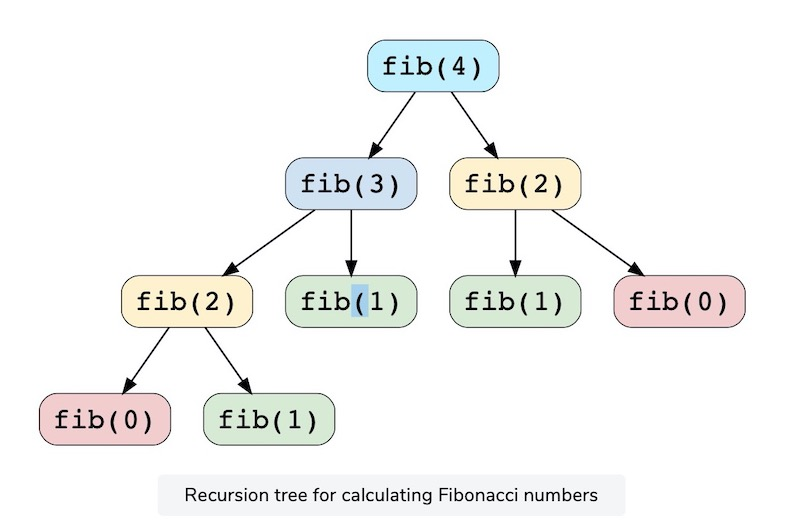
\includegraphics[width=8cm]{fibonacci_recursive_tree}
\end{figure}

\begin{flushleft}

As shown in the diagram above, the nature of this algorithm is recursive.
For example, calculating the 4\textsuperscript{th} element, we need to  calculate the 3\textsuperscript{rd}, 2\textsuperscript{nd} and 1\textsuperscript{st} elements.
This behavior trickles down to the subsequent elements in the sequence and will eventually reach the base case of 0 and 1.
To start classifying this algorithm we can convert the return statement to look like this as a recurrence relation:
$$T(n-1) + T(n-2) + c$$
where c is the number at the bottom of the call stack and takes $O(1)$ to retrieve.

Drawing upon knowledge of the logarithmic relationship between trees and their associated depths, we can make the following assumption:
$$T(n-1) = O(2^{n-1})$$

This is because the depth of a fully populated tree will have $2^{n-1}$ nodes attached to it.
We can plug this into the first equation and get:

$$T(n) = O(2^{n-1}) + O(2^{n-2}) + O(1) \sim O(2^{n})$$
Thus, the classification of this function is $O(2^{n})$, which is exponential and not great for large inputs.

\end{flushleft}

\newpage

\section{Part 1B}

\subsection{Pseudocode | Equation \#2}

\begin{verbatim}
function equation2(int n, int p):
    current_index = current_fib_index(p) # gather the current index (O(1))
    ratio = GOLDEN_RATIO ** (n -p) # raise to the power of n - p (O(n))
    return current_index * ratio # (O(1))

\end{verbatim}

\subsection{Mathematical Analysis | Equation \#2}
\begin{flushleft}
Equation \#2 from the project description is:

$$F_{n} \approx F_{p}\bigg(\frac{1 + \sqrt{5}}{2}\bigg)^{n - p}$$

We need to then use the first equation, which is:
$$ F_{n} = \frac{(1 + \sqrt{5})^{n} + (1 - \sqrt{5})^{n}}{2^{n} \times \sqrt{5}}$$
to get any Fibonacci number, regardless of the position in the sequence.
Therefore, using both equations in conjunction with one another will still result in constant time or $O(1)$.
Also, there is some talk about which implementation of an exponentiating function has a better run time.
In Python, using the math.pow function, it will run in $O(1)$ and will be less precise.
However using the $**$ operator will result in $O(\log(n))$ and will be more precise.
More information can be found \href{https://stackoverflow.com/questions/48839772/why-is-time-complexity-o1-for-powx-y-while-it-is-on-for-xy}{\underline{here}}.
Each of these are running times are based on specific implementations of the Python STL and might not be representative of a language agnostic approach.
An algorithm presented in a class homework assignment uses a linear approach and we will assume this to be our baseline.
Overall, this function should be running in linear time $O(n)$, however, if applied in an actual language, will be the best case of $O(1)$.
\end{flushleft}

\newpage

\subsection{Pseudocode | Equation \#3}

\begin{verbatim}
function equation3(int n):
    current_index = current_fib_index(n+1) # (O(n))
    return current_index * GOLDEN_RATIO # (1)

\end{verbatim}

\subsection{Mathematical Analysis | Equation \#2}
\begin{flushleft}
Equation \#3 from the project description is:
$$F_{n+1} \approx F_{n}\bigg(\frac{1 + \sqrt{5}}{2}\bigg)$$
and we will be using equation \#1 as described above.
Upon further inspection of the aforementioned function, we can still see the need to raise the terms on the numerator to the n\textsuperscript{th} power.
As described in the previous analysis, we are assuming those operations will take at worst $O(n)$.
Therefore, this function will take $O(n)$ to complete.
To confirm the maxim presented in this section, the ratio between $n+1$ and $n-1$ does eventually converge to $\phi = 1.61803$.
\end{flushleft}

\newpage

\section{Part 2}

\subsection{Pseudocode | Largest Sum Subarray}

\begin{verbatim}
function largest_sum(container):
    b = 0, e = 1 # O(1)
    for i from 0 to n-1: # O(n)
        for j from i+1 to n: # O(n)
            if(sum(container[i:j]) > sum(container[b:e])): # O(n) + O(n) = O(2n)
                b = i, e = j # O(1)
    return (b, e) # O(1)
\end{verbatim}

\subsection{Mathematical Analysis | Largest Sum Subarray}
This function is directly pulled from the project description and uses an exhaustive search algorithm.
It requires to search all possible permutations of the indices by using a $O(n^{2})$ search pattern.
To produce the sum of a certain subarray, this will take $O(n)$ time, because this list is not known to be sorted nor in any particular order.
These summations occur once per iteration in the search algorithm.
The instruction count of the above function can be shown as:
$$1 + [O(n) * O(n)] + O(2n) + 1$$
$$2 + O(n^{2}) + O(2n) \implies  O(n^2) + O(2n) + 2 \sim O(n^{2})$$
This function takes $O(n^{2})$ time to complete.
\end{document}
